\documentclass{article}
\usepackage{enumerate}
\usepackage{amsmath}
\usepackage{amssymb}
\usepackage{graphicx}
\usepackage{subfigure}
\usepackage{geometry}
\usepackage{caption}
\usepackage{tikz}
\usepackage{multirow}
\usepackage{array}
\setlength{\parindent}{0pt}

\usepackage{algorithm}
\usepackage{algorithmicx}
\usepackage{algpseudocode}
\renewcommand{\algorithmicrequire}{\textbf{Input:}}
\renewcommand{\algorithmicensure}{\textbf{Output:}}

\geometry{left=3.0cm,right=3.0cm,top=3.0cm,bottom=4.0cm}
\renewcommand{\thesection}{Exercise 9.\arabic{section}}
\title{VE203 Assignment 9}
\author{Liu Yihao 515370910207}
\date{}
\begin{document}
\maketitle

\section{}
\begin{minipage}{0.48\linewidth}
i)
\end{minipage}
\hfill
\begin{minipage}{0.48\linewidth}
ii)
\end{minipage}
\begin{minipage}{0.48\linewidth}
\begin{center}
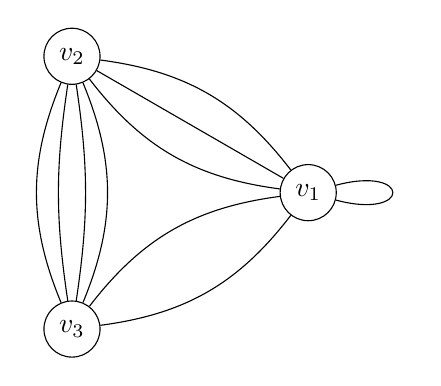
\begin{tikzpicture}[scale=2, bend angle=22.5]
\tikzstyle{every node}=[draw,shape=circle];
\foreach \i in {1,...,3}
{
\path (120*\i-120:1cm) node (v\i) {$v_\i$};
}
\draw
(v1) edge [loop right, every loop/.style={}] (v1) (v1) -- (v2)
(v1) edge [bend left] (v2) (v1) edge [bend right] (v2)
(v1) edge [bend left] (v3) (v1) edge [bend right] (v3)
(v2) edge [bend left] (v3) (v2) edge [bend right] (v3)
(v2) edge [bend left=8.5] (v3) (v2) edge [bend right=8.5] (v3)
;
\end{tikzpicture}
\end{center}
\end{minipage}
\hfill
\begin{minipage}{0.48\linewidth}
\begin{center}
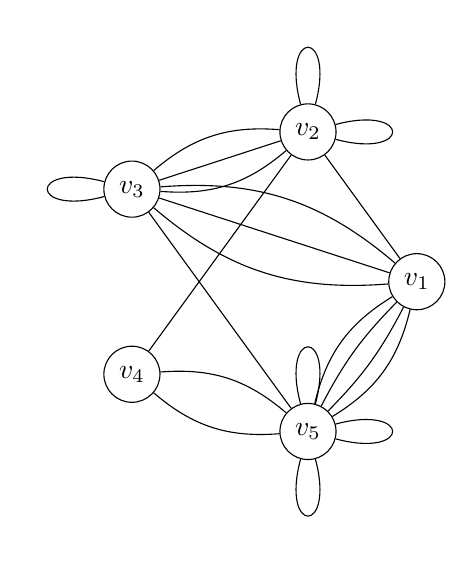
\begin{tikzpicture}[scale=2, bend angle=22.5]
\tikzstyle{every node}=[draw,shape=circle];
\foreach \i in {1,...,5}
{
\path (72*\i-72:1cm) node (v\i) {$v_\i$};
}
\draw
(v1) -- (v2) (v1) -- (v3)
(v1) edge [bend left] (v3) (v1) edge [bend right] (v3)
(v1) edge [bend left] (v5) (v1) edge [bend right] (v5)
(v1) edge [bend left=8.5] (v5) (v1) edge [bend right=8.5] (v5)
(v2) edge [loop above, every loop/.style={}] (v2) 
(v2) edge [loop right, every loop/.style={}] (v2) 
(v2) -- (v3) (v2) -- (v4)
(v2) edge [bend left] (v3) (v2) edge [bend right] (v3)
(v3) edge [loop left, every loop/.style={}] (v3) 
(v3) -- (v5)
(v4) edge [bend left] (v5) (v4) edge [bend right] (v5)
(v5) edge [loop right, every loop/.style={}] (v5) 
(v5) edge [loop above, every loop/.style={}] (v5) 
(v5) edge [loop below, every loop/.style={}] (v5) 
;
\end{tikzpicture}
\end{center}
\end{minipage}


\section{}
\begin{enumerate}[i)]
\item
$$\phi:u_1\to v_1,u_2\to v_4,u_3\to v_2,u_4\to v_5,u_5\to v_3$$
\begin{minipage}{0.1\linewidth}
$$$$
\end{minipage}
\hfill
\begin{minipage}{0.33\linewidth}
\begin{gather*}
\begin{array}{c@{\hspace{2em}}ccccc}
&u_1&u_2&u_3&u_4&u_5
\end{array}
\\
\begin{array}{c}
u_1\\u_2\\u_3\\u_4\\u_5
\end{array}\left(
\begin{array}{c@{\hspace{1.5em}}c@{\hspace{1.5em}}c@{\hspace{1.5em}}c@{\hspace{1.5em}}c}
0&1&0&0&0\\
0&0&1&0&0\\
0&0&0&1&0\\
0&0&0&0&1\\
1&0&0&0&0\\
\end{array}\right)
\end{gather*}
\end{minipage}
\hfill
\begin{minipage}{0.05\linewidth}
$$=$$
\end{minipage}
\hfill
\begin{minipage}{0.33\linewidth}
\begin{gather*}
\begin{array}{c@{\hspace{2em}}ccccc}
&v_1&v_4&v_2&v_5&v_3
\end{array}
\\
\begin{array}{c}
v_1\\v_4\\v_2\\v_5\\v_3
\end{array}\left(
\begin{array}{c@{\hspace{1.5em}}c@{\hspace{1.5em}}c@{\hspace{1.5em}}c@{\hspace{1.5em}}c}
0&1&0&0&0\\
0&0&1&0&0\\
0&0&0&1&0\\
0&0&0&0&1\\
1&0&0&0&0\\
\end{array}\right)
\end{gather*}
\end{minipage}
\hfill
\begin{minipage}{0.15\linewidth}
$$$$
\end{minipage}

So it is an isomorphism.
\item
$$\phi:u_1\to v_1,u_2\to v_3,u_3\to v_2,u_4\to v_5,u_5\to v_4$$
\begin{minipage}{0.1\linewidth}
$$$$
\end{minipage}
\hfill
\begin{minipage}{0.33\linewidth}
\begin{gather*}
\begin{array}{c@{\hspace{2em}}ccccc}
&u_1&u_2&u_3&u_4&u_5
\end{array}
\\
\begin{array}{c}
u_1\\u_2\\u_3\\u_4\\u_5
\end{array}\left(
\begin{array}{c@{\hspace{1.5em}}c@{\hspace{1.5em}}c@{\hspace{1.5em}}c@{\hspace{1.5em}}c}
0&1&0&0&0\\
0&0&1&0&0\\
0&0&0&1&0\\
0&0&0&0&1\\
1&0&0&0&0\\
\end{array}\right)
\end{gather*}
\end{minipage}
\hfill
\begin{minipage}{0.05\linewidth}
$$=$$
\end{minipage}
\hfill
\begin{minipage}{0.33\linewidth}
\begin{gather*}
\begin{array}{c@{\hspace{2em}}ccccc}
&v_1&v_3&v_2&v_5&v_4
\end{array}
\\
\begin{array}{c}
v_1\\v_3\\v_2\\v_5\\v_4
\end{array}\left(
\begin{array}{c@{\hspace{1.5em}}c@{\hspace{1.5em}}c@{\hspace{1.5em}}c@{\hspace{1.5em}}c}
0&1&0&0&0\\
0&0&1&0&0\\
0&0&0&1&0\\
0&0&0&0&1\\
1&0&0&0&0\\
\end{array}\right)
\end{gather*}
\end{minipage}
\hfill
\begin{minipage}{0.15\linewidth}
$$$$
\end{minipage}

So it is an isomorphism.
\item
There are two triangle subgraph $\lbrace u_1,u_2,u_3\rbrace$ and $\lbrace u_5,u_6,u_7\rbrace$ in the first graph,\\
but there isn't any in the second graph, so it isn't an isomorphism.
\item
$$\phi:u_1\to v_3,u_2\to v_1,u_3\to v_2,u_4\to v_5,
	   u_5\to v_6,u_6\to v_8,u_7\to v_7,u_8\to v_4$$

\begin{minipage}{0.47\linewidth}
\begin{gather*}
\begin{array}{c@{\hspace{2em}}cccccccc}
&u_1&u_2&u_3&u_4&u_5&u_6&u_7&u_8
\end{array}
\\
\begin{array}{c}
u_1\\u_2\\u_3\\u_4\\u_5\\u_6\\u_7\\u_8
\end{array}\left(
\begin{array}{c@{\hspace{1.5em}}c@{\hspace{1.5em}}c@{\hspace{1.5em}}c@{\hspace{1.5em}}c@{\hspace{1.5em}}c@{\hspace{1.5em}}c@{\hspace{1.5em}}c}
0&1&1&0&0&0&0&1\\
1&0&1&0&0&1&0&0\\
1&1&0&1&0&0&0&0\\
0&0&1&0&1&0&0&1\\
0&0&0&1&0&1&1&0\\
0&1&0&0&1&0&1&0\\
0&0&0&0&1&1&0&1\\
1&0&0&1&0&0&1&0\\
\end{array}\right)
\end{gather*}
\end{minipage}
\hfill
\begin{minipage}{0.04\linewidth}
$$=$$
\end{minipage}
\hfill
\begin{minipage}{0.47\linewidth}
\begin{gather*}
\begin{array}{c@{\hspace{2em}}cccccccc}
&v_3&v_1&v_2&v_5&v_6&v_8&v_7&v_4
\end{array}
\\
\begin{array}{c}
v_3\\v_1\\v_2\\v_5\\v_6\\v_8\\v_7\\v_4
\end{array}\left(
\begin{array}{c@{\hspace{1.5em}}c@{\hspace{1.5em}}c@{\hspace{1.5em}}c@{\hspace{1.5em}}c@{\hspace{1.5em}}c@{\hspace{1.5em}}c@{\hspace{1.5em}}c}
0&1&1&0&0&0&0&1\\
1&0&1&0&0&1&0&0\\
1&1&0&1&0&0&0&0\\
0&0&1&0&1&0&0&1\\
0&0&0&1&0&1&1&0\\
0&1&0&0&1&0&1&0\\
0&0&0&0&1&1&0&1\\
1&0&0&1&0&0&1&0\\
\end{array}\right)
\end{gather*}
\end{minipage}


So it is an isomorphism.

\end{enumerate}

\section{}
\begin{enumerate}[i)]
\item
For a complete graph, every two vertices are connected.\\
When $n=2k+1,k\in N$, each of the vertices has $2k$ edges, so the graph has an Euler circuit.
When $n=2k,k\in N^+$, each of the vertices has $2k+1$ edges, so the graph hasn't an Euler circuit.
So $n\in\lbrace 2k+1,k\in N\rbrace$
\item
For a wheel graph, the vertex in the center has $n-1$ edges and the other vertices have $n-2$ edges.\\
Since $n-1$ is odd or $n-2$ is odd, the graph never has an Euler circuit.
\item
For a cycle graph, each vertex have two edges, so the graph always has an Euler circuit.
\item
For a cycle graph, each vertex have $n$ edges, when $n$ is even, the graph has an Euler circuit.\\
So $n\in\lbrace 2k+2,k\in N\rbrace$
\end{enumerate}

\section{}
If all simple circuits have even length, for two vertices $u$ and $v$, choosing a vertex $u$ and setting $S=\lbrace v:2|d(u,v)\rbrace$ and $T=\lbrace v:2\not|d(u,v)\rbrace$. Suppose $v_1\in S$ and $v_2\in T$, and $d(v_1,v_2)=d(u,v_1)+d(u,v_2)$ or $d(v_1,v_2)=k-d(u,v_1)-d(u,v_2)$ where k is the length of the simplest circuit containing $u,v_1,v_2$, where k is even. So $d(u,v_1)+d(u,v_2)$ and $k-d(u,v_1)-d(u,v_2)$ are both odd, which means $d(v_1,v_2)$ is odd. So $S$ and $T$ defines a bipartition of the graph.

If a simple circuit have odd length, then the subgraph of the circuit isn't bipartite, so the graph is bipartite only if all simple circuits have even length.

\section{}
Define $sum(V)=the\ addition\ of\ digits\ of\ the\ vertex$, then the bipartition is
$$(\lbrace sum(V)\equiv 0 {\rm(mod\ 2)} \rbrace,\lbrace sum(V)\equiv 1 {\rm(mod\ 2)} \rbrace)$$
For $n=1$, the bipartition of $Q_1$ is $(\lbrace0\rbrace,\lbrace1\rbrace)$\\
For $n=k,k\in N,k>1$, suppose $Q_n$ bipartite for all $n\in N$ and the bipartition is listed above.\\
For $n=k+1$, we have two subgraphs formed from $Q_n$ that adding either 0 or 1 in front of every vertex and then connect them together. We can find that each of the two newly connected vertices are in different partitions since the subgraph adding 1 in the front have totally opposite bipartition. So it is proved.

\section{}
\begin{enumerate}[i)]
\item
The total possible number of edges in a graph containing $n$ vertices is
$$N=\frac{n(n-1)}{2}$$
Since $N_E=N_{E^C}$,
$$N_E=N_{E^C}=\frac{n(n-1)}{4}$$
So only when $n=4m$ or $4m+1,m\in N$, $N_E$ and $N_{E^C}$ are integers.
\item \ \\
\begin{minipage}{0.48\linewidth}
\begin{center}
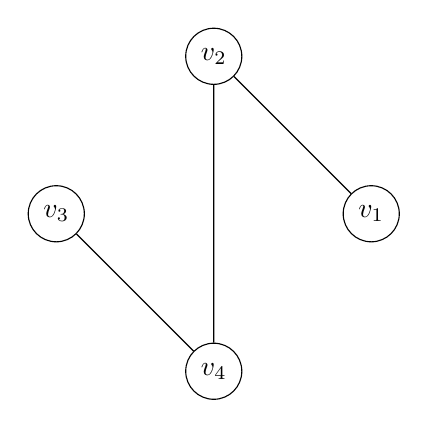
\begin{tikzpicture}[scale=2, bend angle=22.5]
\tikzstyle{every node}=[draw,shape=circle];
\foreach \i in {1,...,4}
{
\path (90*\i-90:1cm) node (v\i) {$v_\i$};
}
\draw
(v1) -- (v2) (v2) -- (v4) (v3) -- (v4);
\end{tikzpicture}
\end{center}
\end{minipage}
\hfill
\begin{minipage}{0.48\linewidth}
\begin{center}
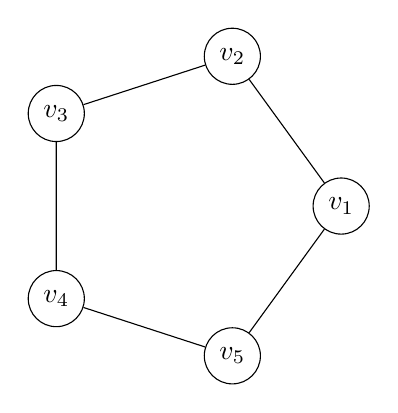
\begin{tikzpicture}[scale=2, bend angle=22.5]
\tikzstyle{every node}=[draw,shape=circle];
\foreach \i in {1,...,5}
{
\path (72*\i-72:1cm) node (v\i) {$v_\i$};
}
\draw
(v1) -- (v2) (v2) -- (v3) (v3) -- (v4) (v4) -- (v5) (v5) -- (v1);
\end{tikzpicture}
\end{center}
\end{minipage}
\begin{center}
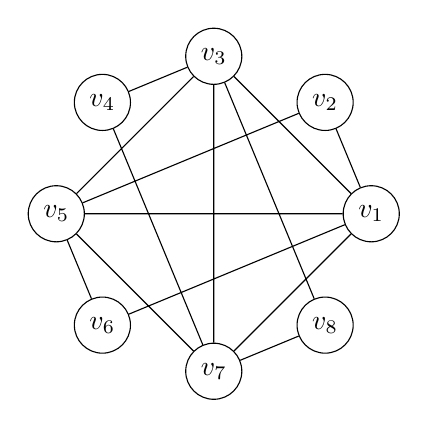
\begin{tikzpicture}[scale=2, bend angle=22.5]
\tikzstyle{every node}=[draw,shape=circle];
\foreach \i in {1,...,8}
{
\path (45*\i-45:1cm) node (v\i) {$v_\i$};
}
\draw
(v1) -- (v2) (v3) -- (v4) (v5) -- (v6) (v7) -- (v8)
(v1) -- (v3) (v3) -- (v5) (v5) -- (v7) (v7) -- (v1)
(v2) -- (v5) (v4) -- (v7) (v6) -- (v1) (v8) -- (v3)
(v1) -- (v5) (v3) -- (v7);
\end{tikzpicture}
\end{center}
\end{enumerate}

\section{}
\begin{enumerate}[i)]
\item
Suppose the addition of a single edge will never produce a Hamilton circuit in $H$, but if we add edges to form a complete graph, there must exist a Hamilton circuit in $H$, which reaches a contradiction. So it is proved.
\item
Since there exists a Hamilton circuit in $H$, then we can remove one added edge in the circuit so that the vertices on the two sides of the edge are not adjacent, then we get a Hamilton path in $H$.
\item
Since in $G$, $deg(x)+deg(y)>n$, and $deg_H(v)\geqslant deg_G(v)$, so $deg(v_1)+deg(v_n)>n$ in $H$.\\
We know $n-deg(v_n)<deg(v_1)$, and $n-deg(v_n)$ is the number of vertices not adjacent to $v_n$, so there are at most $deg(v_1)$ vertices not adjacent to $v_n$.
\item
Since $S$ is the set of vertices preceding each vertex adjacent to $v_1$, so $S$ contains $deg(v_1)$ vertices.\\
Since $v_1,...,v_n$ is a Hamilton path, $v_n$ is the last vertex, $v_{n+1}$ doesn't exists. So $v_n\not\in S$.
\item
Since there are $deg(v_1)$ vertices in $S$ and $deg(v_n)$ vertices adjacent to $v_n$, and $deg(v_1)+deg(v_n)>n$, according to the Pigeonhole Principle, there is at least a vertex $v_k$ both in $S$ and adjacent to $v_n$. So $v_k\in S$ and $v_k$ is adjacent to $v_n$, then according to the definition of $S$, $v_{k+1}$ is adjacent to $v_1$. Since $v_1,...,v_n$ is a Hamilton path, $v_k$ is adjacent to $v_{k+1}$. So $v_1$ and $v_{k+1}$ and $v_k$ and $v_n$ are connected.
\item
There are edges between $v_1,v_2,...,v_{k-1},v_k,v_n,v_{n-1},...,v_{k+1},v_1$, so it is a Hamilton circuit, which reaches a contradiction with the suppose in part iii). So the Ore's Theorem holds.
\end{enumerate}


\section{}
0$\rm^{nd}$ Iteration:\\
$S_0=\emptyset$\\

1$\rm^{st}$ Iteration:\\
$S_{1}=\lbrace U \rbrace$\\
$U:0$, $D:7\ (U)$, $E:10\ (U)$, $Q:4\ (U)$, $Z:6\ (U)$\\

2$\rm^{nd}$ Iteration:\\
$S_{2}=\lbrace U,D \rbrace$\\
$U:0$, $D:7\ (U)$, $E:10\ (U)$, $Q:4\ (U)$, $Z:6\ (U)$, $C:17\ (U,D)$\\

3$\rm^{rd}$ Iteration:\\
$S_{3}=\lbrace U,D,E \rbrace$\\
$U:0$, $D:7\ (U)$, $E:10\ (U)$, $Q:4\ (U)$, $Z:6\ (U)$, $C:17\ (U,D)$, $F:20\ (U,E)$\\

4$\rm^{th}$ Iteration:\\
$S_{4}=\lbrace U,D,E,Q \rbrace$\\
$U:0$, $D:7\ (U)$, $E:10\ (U)$, $Q:4\ (U)$, $Z:6\ (U)$, $C:17\ (U,D)$, $F:14\ (U,Q)$, $P:9\ (U,Q)$, $T:11\ (U,Q)$\\

5$\rm^{th}$ Iteration:\\
$S_{5}=\lbrace U,D,E,Q,Z \rbrace$\\
$U:0$, $D:7\ (U)$, $E:10\ (U)$, $Q:4\ (U)$, $Z:6\ (U)$, $C:17\ (U,D)$, $F:14\ (U,Q)$, $P:9\ (U,Q)$, $T:11\ (U,Q)$\\

6$\rm^{th}$ Iteration:\\
$S_{6}=\lbrace U,D,E,Q,Z,C \rbrace$\\
$U:0$, $D:7\ (U)$, $E:10\ (U)$, $Q:4\ (U)$, $Z:6\ (U)$, $C:17\ (U,D)$, $F:14\ (U,Q)$, $P:9\ (U,Q)$, $T:11\ (U,Q)$, $B:25\ (U,D,C)$\\

7$\rm^{th}$ Iteration:\\
$S_{7}=\lbrace U,D,E,Q,Z,C,F \rbrace$\\
$U:0$, $D:7\ (U)$, $E:10\ (U)$, $Q:4\ (U)$, $Z:6\ (U)$, $C:17\ (U,D)$, $F:14\ (U,Q)$, $P:9\ (U,Q)$, $T:11\ (U,Q)$, $B:25\ (U,D,C)$, $G:20\ (U,Q,F)$, $X:23\ (U,Q,F)$\\

8$\rm^{th}$ Iteration:\\
$S_{8}=\lbrace U,D,E,Q,Z,C,F,P \rbrace$\\
$U:0$, $D:7\ (U)$, $E:10\ (U)$, $Q:4\ (U)$, $Z:6\ (U)$, $C:16\ (U,Q,P)$, $F:14\ (U,Q)$, $P:9\ (U,Q)$, $T:11\ (U,Q)$, $B:25\ (U,D,C)$, $G:20\ (U,Q,F)$, $X:23\ (U,Q,F)$, $O:15\ (U,Q,P)$, $S:15\ (U,Q,P)$\\

9$\rm^{th}$ Iteration:\\
$S_{9}=\lbrace U,D,E,Q,Z,C,F,P,T \rbrace$\\
$U:0$, $D:7\ (U)$, $E:10\ (U)$, $Q:4\ (U)$, $Z:6\ (U)$, $C:16\ (U,Q,P)$, $F:14\ (U,Q)$, $P:9\ (U,Q)$, $T:11\ (U,Q)$, $B:25\ (U,D,C)$, $G:20\ (U,Q,F)$, $X:14\ (U,Q,T)$, $O:15\ (U,Q,P)$, $S:15\ (U,Q,P)$\\

10$\rm^{th}$ Iteration:\\
$S_{10}=\lbrace U,D,E,Q,Z,C,F,P,T,B \rbrace$\\
$U:0$, $D:7\ (U)$, $E:10\ (U)$, $Q:4\ (U)$, $Z:6\ (U)$, $C:16\ (U,Q,P)$, $F:14\ (U,Q)$, $P:9\ (U,Q)$, $T:11\ (U,Q)$, $B:25\ (U,D,C)$, $G:20\ (U,Q,F)$, $X:14\ (U,Q,T)$, $O:15\ (U,Q,P)$, $S:15\ (U,Q,P)$, $A:31\ (U,D,C,B)$\\

11$\rm^{th}$ Iteration:\\
$S_{11}=\lbrace U,D,E,Q,Z,C,F,P,T,B,G \rbrace$\\
$U:0$, $D:7\ (U)$, $E:10\ (U)$, $Q:4\ (U)$, $Z:6\ (U)$, $C:16\ (U,Q,P)$, $F:14\ (U,Q)$, $P:9\ (U,Q)$, $T:11\ (U,Q)$, $B:25\ (U,D,C)$, $G:20\ (U,Q,F)$, $X:14\ (U,Q,T)$, $O:15\ (U,Q,P)$, $S:15\ (U,Q,P)$, $A:31\ (U,D,C,B)$, $H:31\ (U,Q,F,G)$\\

12$\rm^{th}$ Iteration:\\
$S_{12}=\lbrace U,D,E,Q,Z,C,F,P,T,B,G,X \rbrace$\\
$U:0$, $D:7\ (U)$, $E:10\ (U)$, $Q:4\ (U)$, $Z:6\ (U)$, $C:16\ (U,Q,P)$, $F:14\ (U,Q)$, $P:9\ (U,Q)$, $T:11\ (U,Q)$, $B:25\ (U,D,C)$, $G:20\ (U,Q,F)$, $X:14\ (U,Q,T)$, $O:15\ (U,Q,P)$, $S:15\ (U,Q,P)$, $A:31\ (U,D,C,B)$, $H:17\ (U,Q,T,X)$, $W:23\ (U,Q,T,X)$\\

13$\rm^{th}$ Iteration:\\
$S_{13}=\lbrace U,D,E,Q,Z,C,F,P,T,B,G,X,O \rbrace$\\
$U:0$, $D:7\ (U)$, $E:10\ (U)$, $Q:4\ (U)$, $Z:6\ (U)$, $C:16\ (U,Q,P)$, $F:14\ (U,Q)$, $P:9\ (U,Q)$, $T:11\ (U,Q)$, $B:24\ (U,Q,P,O)$, $G:20\ (U,Q,F)$, $X:14\ (U,Q,T)$, $O:15\ (U,Q,P)$, $S:15\ (U,Q,P)$, $A:31\ (U,D,C,B)$, $H:17\ (U,Q,T,X)$, $W:23\ (U,Q,T,X)$, $N:20\ (U,Q,P,O)$, $Y:19\ (U,Q,P,O)$\\

14$\rm^{th}$ Iteration:\\
$S_{14}=\lbrace U,D,E,Q,Z,C,F,P,T,B,G,X,O,S \rbrace$\\
$U:0$, $D:7\ (U)$, $E:10\ (U)$, $Q:4\ (U)$, $Z:6\ (U)$, $C:16\ (U,Q,P)$, $F:14\ (U,Q)$, $P:9\ (U,Q)$, $T:11\ (U,Q)$, $B:24\ (U,Q,P,O)$, $G:20\ (U,Q,F)$, $X:14\ (U,Q,T)$, $O:15\ (U,Q,P)$, $S:15\ (U,Q,P)$, $A:31\ (U,D,C,B)$, $H:17\ (U,Q,T,X)$, $W:23\ (U,Q,T,X)$, $N:20\ (U,Q,P,O)$, $Y:18\ (U,Q,P,S)$, $R:22\ (U,Q,P,S)$\\

15$\rm^{th}$ Iteration:\\
$S_{15}=\lbrace U,D,E,Q,Z,C,F,P,T,B,G,X,O,S,A \rbrace$\\
$U:0$, $D:7\ (U)$, $E:10\ (U)$, $Q:4\ (U)$, $Z:6\ (U)$, $C:16\ (U,Q,P)$, $F:14\ (U,Q)$, $P:9\ (U,Q)$, $T:11\ (U,Q)$, $B:24\ (U,Q,P,O)$, $G:20\ (U,Q,F)$, $X:14\ (U,Q,T)$, $O:15\ (U,Q,P)$, $S:15\ (U,Q,P)$, $A:31\ (U,D,C,B)$, $H:17\ (U,Q,T,X)$, $W:23\ (U,Q,T,X)$, $N:20\ (U,Q,P,O)$, $Y:18\ (U,Q,P,S)$, $R:22\ (U,Q,P,S)$, $M:38\ (U,D,C,B,A)$\\

16$\rm^{th}$ Iteration:\\
$S_{16}=\lbrace U,D,E,Q,Z,C,F,P,T,B,G,X,O,S,A,H \rbrace$\\
$U:0$, $D:7\ (U)$, $E:10\ (U)$, $Q:4\ (U)$, $Z:6\ (U)$, $C:16\ (U,Q,P)$, $F:14\ (U,Q)$, $P:9\ (U,Q)$, $T:11\ (U,Q)$, $B:24\ (U,Q,P,O)$, $G:20\ (U,Q,F)$, $X:14\ (U,Q,T)$, $O:15\ (U,Q,P)$, $S:15\ (U,Q,P)$, $A:31\ (U,D,C,B)$, $H:17\ (U,Q,T,X)$, $W:23\ (U,Q,T,X)$, $N:20\ (U,Q,P,O)$, $Y:18\ (U,Q,P,S)$, $R:22\ (U,Q,P,S)$, $M:38\ (U,D,C,B,A)$, $I:27\ (U,Q,T,X,H)$\\

17$\rm^{th}$ Iteration:\\
$S_{17}=\lbrace U,D,E,Q,Z,C,F,P,T,B,G,X,O,S,A,H,W \rbrace$\\
$U:0$, $D:7\ (U)$, $E:10\ (U)$, $Q:4\ (U)$, $Z:6\ (U)$, $C:16\ (U,Q,P)$, $F:14\ (U,Q)$, $P:9\ (U,Q)$, $T:11\ (U,Q)$, $B:24\ (U,Q,P,O)$, $G:20\ (U,Q,F)$, $X:14\ (U,Q,T)$, $O:15\ (U,Q,P)$, $S:15\ (U,Q,P)$, $A:31\ (U,D,C,B)$, $H:17\ (U,Q,T,X)$, $W:23\ (U,Q,T,X)$, $N:20\ (U,Q,P,O)$, $Y:18\ (U,Q,P,S)$, $R:22\ (U,Q,P,S)$, $M:38\ (U,D,C,B,A)$, $I:27\ (U,Q,T,X,H)$, $V:27\ (U,Q,T,X,W)$\\

So the length is 23 and the path is $(U,Q,T,X,W)$\\



\end{document}
